\section{Results}

\subsection{False-Positive Baseline (Deterministic)}

I tested the deterministic pipeline (Tiers~1--2, no AI) against 391 real citations from three sources. Every citation flagged as \textit{suspicious} or \textit{invalid} is a false positive.

\begin{table}[H]
\centering
\caption{False-positive rate on real citations (deterministic validation, no AI).}
\label{tab:fpr}
\begin{tabular}{@{}lrrrrrr@{}}
\toprule
\textbf{Dataset} & \textbf{$n$} & \textbf{Valid} & \textbf{Warning} & \textbf{Suspicious} & \textbf{Invalid} & \textbf{FPR} \\
\midrule
arXiv CS (2024)  & 285 &   2 & 283 & 0 & 0 & 0.0\% \\
CrossRef random  &  96 &  94 &   2 & 0 & 0 & 0.0\% \\
Nature article   &  10 &   5 &   5 & 0 & 0 & 0.0\% \\
\midrule
\textbf{Total}   & \textbf{391} & 101 & 290 & 0 & 0 & \textbf{0.0\%} \\
\bottomrule
\end{tabular}
\end{table}

Zero real citations were flagged as suspicious or invalid. The Wilson 95\% confidence interval for 0/391 is $[0.0\%,\; 0.96\%]$---I can claim less than 1\% FPR with 95\% confidence, but not exactly zero.

\begin{figure}[!h]
  \centering
  \caption{\emph{Citation Validator} output on a mixed test bibliography.}
  \label{fig:validator-output}
  \vspace{0.5\baselineskip}
  \fbox{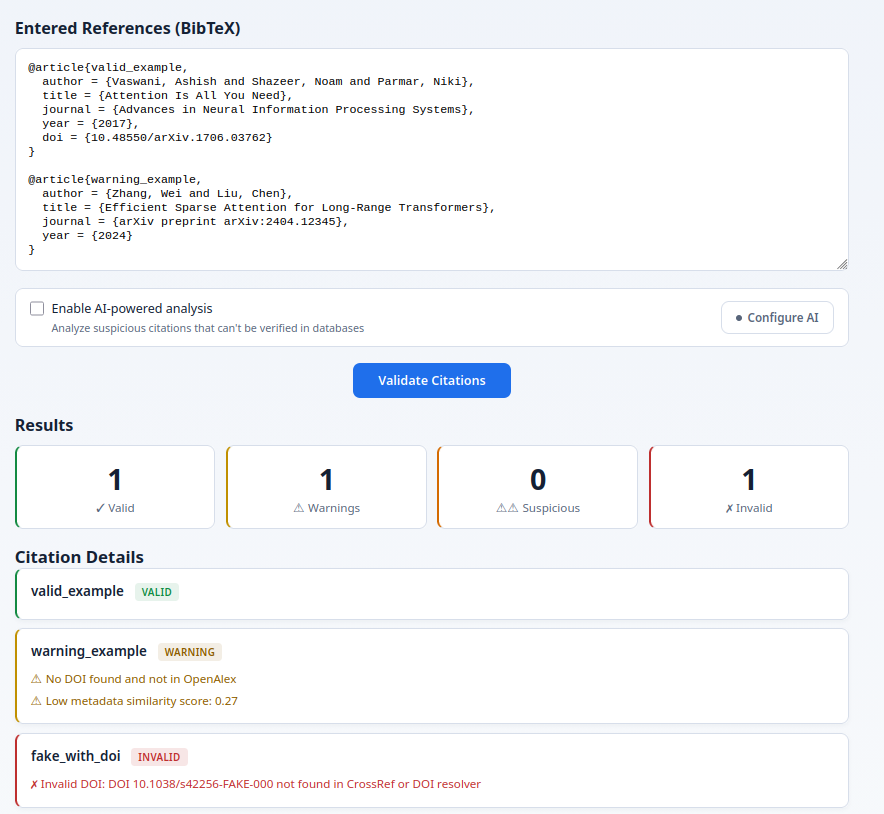
\includegraphics[width=0.81\textwidth]{figures/fig3.png}}
  \vspace{0.75\baselineskip}
  \caption*{%
    \textbf{Note:} A citation with a valid DOI receives \textit{valid} status (green). A citation absent from databases receives \textit{warning} (yellow). A citation with a fabricated DOI receives \textit{invalid} (red). Only \textit{suspicious} and \textit{invalid} statuses count as flags.
  }
\end{figure}
\FloatBarrier

Two features of these results warrant comment. First, 290 of 391 citations (74\%) received \textit{warning} status, meaning the validator could not verify them but did not flag them. This is by design: the \textit{warning} category absorbs the uncertainty that would otherwise produce false positives. Second, the arXiv dataset---where 283 of 285 citations landed at \textit{warning}---represents the hardest case for false-positive avoidance. These are legitimate preprints that mostly lack DOIs and are often absent from OpenAlex and Semantic Scholar. The validator's restraint on this dataset is the direct consequence of the escalation fix described in the Methods.

\subsection{Fake-Citation Detection (Deterministic)}

I tested the same deterministic pipeline against 500 fabricated citations across five deception strategies. Every fake \emph{not} flagged as \textit{suspicious} or \textit{invalid} is a false negative.

\begin{table}[H]
\centering
\caption{Detection rate on fabricated citations (deterministic validation, no AI).}
\label{tab:detection}
\begin{tabular}{@{}llrrr@{}}
\toprule
\textbf{Category} & \textbf{DOI?} & \textbf{$n$} & \textbf{Detected} & \textbf{Rate} \\
\midrule
Stolen DOI    & Yes         & 100 & 100 & 100.0\% \\
Plausible     & Yes (fake)  & 100 & 100 & 100.0\% \\
Ansari 100    & Mostly no   & 100 &   4 &   4.0\% \\
Nonsense      & No          & 100 &  25 &  25.0\% \\
Frankenstein  & No          & 100 &   0 &   0.0\% \\
\midrule
\textbf{Total} &            & \textbf{500} & \textbf{229} & \textbf{45.8\%} \\
\bottomrule
\end{tabular}
\end{table}

The pattern is stark: \textbf{detection depends entirely on whether the citation has a DOI to check.}

\begin{itemize}
  \item \textbf{With DOI} (Stolen DOI + Plausible): 200/200 = 100\%. DOI resolution either fails (fake DOI $\to$ \textit{invalid}) or returns mismatched metadata (real DOI + wrong title $\to$ \textit{suspicious}).
  \item \textbf{Without DOI} (Ansari + Frankenstein + Nonsense): 29/300 = 9.7\%. The validator searches OpenAlex and Semantic Scholar, finds no match, and classifies the citation as \textit{warning}---not \textit{suspicious}.
\end{itemize}

This is the symmetric consequence of the escalation fix that yielded 0\% FPR. The same design decision that prevents flagging legitimate unindexed citations also prevents flagging fabricated ones. The validator correctly says ``I cannot verify this'' but cannot say ``this is fake.'' This is not a bug. It is the fundamental limit of deterministic detection without DOIs.

The 25\% detection rate on Nonsense fakes comes from the heuristic detectors: future publication years and other obvious anomalies that trigger escalation independent of database lookups. The 4\% on Ansari~100 reflects the small number of those citations that happened to carry checkable DOIs.

\subsection{AI-Assisted Detection}

\subsubsection{Free Tier: Gemini 2.5 Flash}

I ran the Ansari~100 dataset through the full pipeline with Gemini 2.5 Flash as the Tier~3 AI provider. The deterministic tiers ran first; Gemini then analyzed all citations with \textit{warning} or \textit{suspicious} status.

\begin{table}[H]
\centering
\caption{Detection on Ansari~100 fakes: deterministic vs.\ deterministic + Gemini.}
\label{tab:gemini-fakes}
\begin{tabular}{@{}lrrrr@{}}
\toprule
\textbf{Pipeline} & \textbf{Detected} & \textbf{Missed} & \textbf{Rate} & \textbf{Cost} \\
\midrule
Deterministic only         &   4 & 96 &  4.0\% & \$0 \\
Deterministic + Gemini     &  94 &  6 & 94.0\% & \$0 \\
\bottomrule
\end{tabular}
\end{table}

Gemini correctly escalated 90 of 96 \textit{warning} citations to \textit{suspicious}. Six fakes remained at \textit{warning} (false negatives). The combined pipeline achieved 94\% recall with an F1 score of 0.97, at zero cost via Gemini's free tier (1 million tokens/day). Total token usage was 58{,}917 tokens (589 average per citation)---well within the daily allowance. At this rate, a journal editor could analyze approximately 1{,}700 citations per day at no cost.

\subsubsection{Paid Tier: Claude Sonnet 4}

I ran the identical experiment with Claude Sonnet 4 (Anthropic) as the AI provider, at a cost of approximately \$0.50 per 100 citations. I then ran both providers on a second dataset---the Frankenstein fakes (real authors paired with fabricated titles, no DOIs)---to test whether the Ansari results would replicate.

\begin{table}[H]
\centering
\caption{AI provider comparison across two fabricated-citation datasets.}
\label{tab:ai-comparison}
\begin{tabular}{@{}llrrrrl@{}}
\toprule
\textbf{Dataset} & \textbf{Provider} & \textbf{Detection} & \textbf{Errors} & \textbf{Time (s)} & \textbf{Cost} \\
\midrule
\multirow{3}{*}{Ansari 100}
  & Deterministic      &   4\% & 0 &  94 & \$0 \\
  & Gemini 2.5 Flash   &  94\% & 0 & 136 & \$0 \\
  & Claude Sonnet 4    &  82\% & 6 & 429 & \textasciitilde\$0.50 \\
\midrule
\multirow{3}{*}{Frankenstein 100}
  & Deterministic      &   0\% & 0 &  92 & \$0 \\
  & Gemini 2.5 Flash   & 100\% & 0 & 120 & \$0 \\
  & Claude Sonnet 4    & 100\% & 0 & 343 & \textasciitilde\$0.50 \\
\bottomrule
\end{tabular}
\end{table}

On the Frankenstein dataset, both providers achieved 100\% detection with zero errors. On the Ansari dataset---real hallucinations from published NeurIPS papers, which represent harder and more diverse fakes---Gemini detected 94\% versus Claude's 82\%. Claude's server errors (6 HTTP~529 responses on Ansari, 0 on Frankenstein) appear to have been transient. Even excluding those errors, Claude's judgment accuracy on successful Ansari calls was 78/90 = 86.7\%, below Gemini's 90/96 = 93.75\%.

Across both datasets, Gemini was consistently faster (120--136s vs.\ 343--429s) and had zero errors. The free tier matched or exceeded the paid tier on every metric.

This finding is more robust than a single-dataset comparison, but its limits are real: two datasets ($n=200$ total), a single prompt per provider, and both datasets consist of fabricated citations without DOIs. The claim is not that Gemini is categorically superior to Claude. The claim is that the free tier is \emph{sufficient}---and that the access barrier imposed by paid APIs is not justified by superior performance on this task.

\subsection{The Precision Collapse}

The results above show that AI dramatically improves recall on fabricated citations. The critical question is whether it preserves precision on real ones. I ran Gemini on the real-citation datasets from Table~\ref{tab:fpr}.

\begin{table}[H]
\centering
\caption{False-positive rate with and without Gemini AI on real citations.}
\label{tab:fpr-ai}
\begin{tabular}{@{}lrrr@{}}
\toprule
\textbf{Dataset} & \textbf{$n$} & \textbf{Deterministic FPR} & \textbf{+ Gemini FPR} \\
\midrule
arXiv CS (285 real, mostly no DOI)    & 285 & 0.0\% & \textbf{72.3\%} \\
CrossRef random (96 real, mostly with DOI) &  96 & 0.0\% & 2.1\% \\
\bottomrule
\end{tabular}
\end{table}

Gemini flagged 206 of 285 real arXiv citations as suspicious. These are legitimate preprints---the same citations that deterministic validation correctly classified as \textit{warning}. On CrossRef citations, where most entries have DOIs and are well-indexed, Gemini's FPR was only 2.1\% (2/96: a Korean-language paper and an 1885 publication).

The contrast is sharp. On fabricated citations, Gemini raises detection from 4\% to 94\%. On real preprints without DOIs, it raises the false-positive rate from 0\% to 72.3\%. The weighted FPR across all 381 real citations Gemini analyzed is $(206 + 2)/(285 + 96) = 54.6\%$.

\subsection{Summary of Results}

Table~\ref{tab:summary} presents the complete picture.

\begin{table}[H]
\centering
\caption{Summary: what works and what does not.}
\label{tab:summary}
\begin{tabular}{@{}p{0.45\textwidth}p{0.45\textwidth}@{}}
\toprule
\textbf{What works} & \textbf{What does not (yet)} \\
\midrule
Deterministic on DOI citations: 0\% FPR, 100\% detection &
Deterministic on non-DOI citations: 0\% FPR but only 4--25\% detection \\[0.5em]
Gemini on fakes: 94\% detection at \$0 &
Gemini on real preprints: 72\% FPR---unusable without selective routing \\[0.5em]
Free outperforms paid (Gemini $>$ Claude on this task) &
AI applied unconditionally destroys precision \\
\bottomrule
\end{tabular}
\end{table}

\noindent The tool is most reliable in deterministic mode: zero false positives, perfect detection on DOI-bearing citations, and honest \textit{warning} on everything else. AI improves recall but requires selective routing---only citations with multiple red flags should be escalated, not every unverifiable citation.

\enlargethispage{\baselineskip}
